\section{Week 4 Dangers of Concurrency}

Concurrent programming creates the possibility for new kinds of errors.

\subsection{Parallelism Correctness Criteria}

\begin{description}
  \item[Race Condition] not enough synchronization, possibility of errors that should not happen according to the program logic. Knowledge of 'what is correct' is necessary to specify the error.
  \item[Data Race] actual occurence of an 'illegal' operation on memory in a concurrent context. Several threads access the same variable/array in memory, at least one write acceess, without synchronization. Forbidden in Java Spec, results undefined.
  \item[Deadlock] If two threads wait for each other when trying to lock 2 resources in reverse order. Can be identified with a resource graph. 
  \begin{figure}
    \centering
    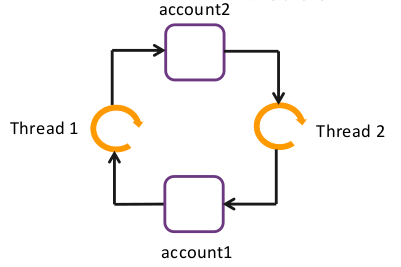
\includegraphics[width=6cm]{res/04-resource-graph.png}
    \caption{Resource Graph identifies Deadlocks}
  \end{figure}
  \textit{Solution:} define an order for locking OR use more coarse granular locking when ordering does not make sense.
  \item[Livelock] Same as deadlock, but executing instructions while waiting. 
  \item[Starvation] When no fairness is in place, one thread runs the risk of having to wait 'forever' to access a resource.
\end{description}

\noindent
\textit{Ergo:} For a program to be formally correct in a parallel execution it must have \textbf{no race conditions, no deadlocks and no starvation.}

\begin{figure}
  \centering
  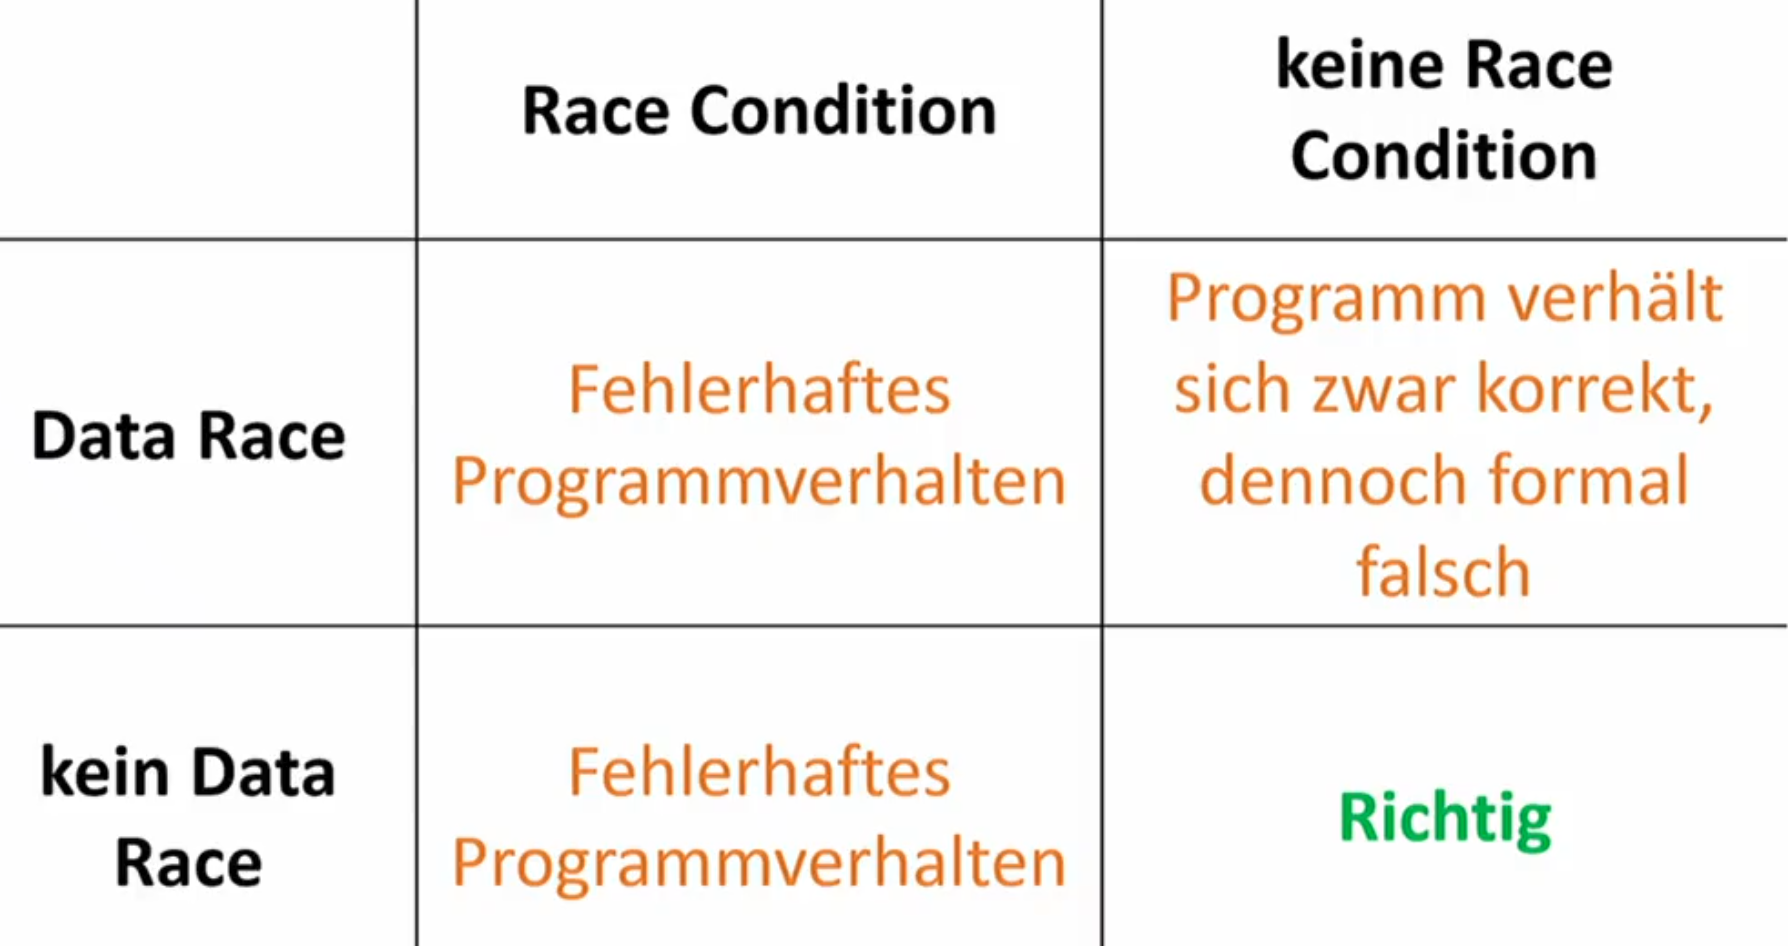
\includegraphics[width=8cm]{res/04-datarace-raceconditions.png}
  \caption{Data Races and Race Conditions}
\end{figure}

\subsection{No Synchronization needed}
\begin{description}
  \item[Immutability] Read only variables
  \item[Thread Confinement] Object belongs to one thread only at any point in time.
  \item[Object Confinement] encapsulation of inner objects by synchronizing all access via an outer class. 
\end{description}

\subsection{Thread Safety}
The avoidance of data races. \textit{When no sharing is intended}, give each thread a private copy of the relevant data.
\textit{When sharing is important}, provide explicit synchronization to make certain the program behaves in a deterministic manner.

\begin{figure}[H]
  \centering
  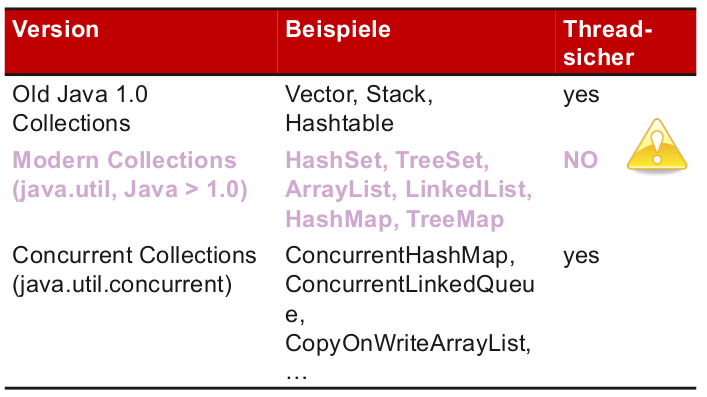
\includegraphics[width=8cm]{res/04-thread-safe-collections.png}
  \caption{Java Collections}
\end{figure}

New approach: provide synchronization only when explicitly needed.
